\chapter{Tools of low--dimensional topology}
\label{chapter:problem}

Given a smooth, closed 3--manifold $M$, there are infinitely many 4--manifolds with boundary $M$.
For example, consider $M=S^3$.
Removing a 4--ball from any 4--manifold $W$ produces a 4--manifold with $S^3$ boundary.
We therefore do not ensure that the constructed 4--manifold has any properties other than a specified boundary, so our construction prioritizes easy verification that the constructed 4--manifold's boundary is exactly $M$.
This is done by setting $W=M\times \Ilit$, so $W$ has boundary 
\[
	\pd W = (M\times\{0\}) \cup (M\times\{1\}) = M_0 \cup M_1.
\]
We then attach stratified handles to the boundary of $W$ away from $M_0$ until only $M_0$ remains.


\section{Handles}
\label{section:problem-handles}

The concept of a stratified handle attachment needs some explanation.
First, we define attachment of topological spaces, and use that language to define handle attachment.


\begin{defn}[Attachment]
	Let $X$ and $Y$ be topological spaces, $A\subset X$ a subspace, and $f:A\to Y$ a continuous map.
	We define a relation $\sim$ by putting $f(x)\sim x$ for every $x$ in $A$.
	Denote the quotient space $X\sqcup Y/\sim$ by $X\cup_f Y$.
	We call the map $f$ the \emph{attaching map}.  
	We say that $X$ is \emph{attached} or \emph{glued} to $Y$ over $A$.
	A space obtained through attachment is called an \emph{adjunction space} or \emph{attachment space}.
	
	Alternatively, we let $A$ be a topological space and let $i_X:A\to X$, $i_Y:A\to Y$ be inclusions.
	Here, the adjunction is formed by taking $i_X(a)\sim i_Y(a)$ for every $a\in A$ and we denote the adjunction space by $X\cup_A Y$.
\end{defn}

\begin{defn}[Handle]
	\label{def:handle}
	Take $n=\lambda+\mu$ and $M$ a smooth $n$--manifold with nonempty boundary $\pd M$.
	Let $D^\lambda$ be the closed $\lambda$--disk and put $H^\lambda = D^\lambda\times D^\mu$.
	Let $\varphi:\pd D^\lambda\times D^\mu\to\pd M$ be an embedding and an attaching map between $M$ and $H^\lambda$.
	The attached space $H^\lambda$ is an \emph{$n$--dimensional $\lambda$--handle}, abbreviated \emph{$(n,\lambda)$--handle}, and $M\cup_\varphi H^\lambda$ is the result of an \emph{$n$--dimensional $\lambda$--handle attachment}, abbreviated \emph{$(n,\lambda)$--handle attachment}.
\end{defn}

Handle attachment is defined for smooth manifolds, but the resulting attachment space is not a smooth manifold.
Rather, the result is a stratified manifold.

\section{Stratification}
\label{section:problem-stratification}

We define stratification using the definition from \cite{wein94}.

\begin{defn}[Stratification]
	$X$ is a \emph{filtered space} on a finite partially ordered indexing set $S$ if 
	\begin{enumerate}
		\item there is a closed subset $X_s$ for each $s\in S$,
		\item $s\leq s'$ implies that $X_s\subset X_{s'}$, and
		\item the inclusions $X_s \into X_{s'}$ satisfy the homotopy lifting property.
	\end{enumerate}
	The $X_s$ are the \emph{closed strata} of $X$, and the differences
	$$X^s = X_s\setminus \bigcup_{r < s} X_r$$
	are \emph{pure strata}.
	
	
	A \emph{filtered map} between spaces filtered over the same indexing set is a continuous function $f:X\to Y$ such that $f(X_s)\subset Y_s$, and such a map is \emph{stratified} if $f(X^s) \subset Y^s$.
	This leads to definitions of stratified homotopy, therefore stratified homotopy equivalence.
\end{defn}

Immediate examples of stratified manifolds are manifolds with boundary and manifolds with corners.
Many handles (e.g.\ $\Ilit\times\Ilit$) are manifolds with corners, and the result of a smooth handle attachment is a manifold with corners at $\varphi(\pd D^\lambda \times \pd D^\mu)$.
Hence both are stratified manifolds.

A \emph{stratified handle attachment} is a handle attachment where the handle, the manifold to which we attach the handle, and the attaching map are each stratified.
The main distinctions between stratified handle attachment and handle attachment are:
\begin{enumerate}
	\item the handle is necessarily stratified, though the stratification is not necessarily induced by the corners that occur in the standard formation of a handle as the Cartesian product of a pair of disks,
	
	\item the manifold to which we attach the handle is necessarily stratified, and
	
	\item the attaching map ensures that there is a coherent identification between the strata of the handle and the strata of the manifold (i.e.\ the stratification of the resulting attachment space is well-defined).
\end{enumerate}


\section{Handlebodies}
\label{section:problem-handlebodies}

Handlebodies are objects central to arguments found near the end of Chapters \ref{chapter:smooth} and \ref{chapter:triangulation}.
A handlebody is formed by attaching some number of $(n,\lambda)$--handles to an $(n,0)$--handle.
The name is evoked by the type of handlebody that we examine in this section: the (3,1)--handlebody.

\begin{defn}
	A connected $n$--manifold $M$ that has a handle decomposition consisting of exactly one 0--handle and $g$ $\lambda$--handles is called an \emph{$(n,\lambda)$--handlebody} of \emph{genus} $g$.
	
	Let $V$ be an $(n,1)$--handlebody of genus $g$.
	A simple closed curve in $\pd V$ is called \emph{essential} if it is not homotopic to a point.
	A simple closed curve $J$ in $\pd V$ that is essential in $\pd V$ and that bounds a 2--disc in $V$ is called a \emph{meridian}.
	The properly embedded disc in $V$ that has boundary $J$ is called a \emph{meridinal disc}.
	
	The special case of the oriented genus 1 $(m,1)$--handlebody is called a \emph{solid torus}.
	More generally, any space that is homeomorphic to $S^1\times D^{n-1}$ is called a \emph{solid $n$--torus}.
	In our most common case of $n=3$, we just say that $S^1\times D^2$ is a \emph{solid torus}.
	A simple closed curve $J$ in the boundary of a solid torus that intersects a meridian at a single point is called a \emph{longitude}.
	A longitude is essential in a solid torus and there are infinitely many isotopy classes of longitudes, but there is exactly one isotopy class of meridians.
\end{defn}

We apply handlebodies to 3--manifold classification through Heegaard splittings.
%When you build a 3--manifold by gluing a pair of genus $g$ (3,1)--handlebodies together over their boundaries, you have formed a Heegaard splitting.

\begin{defn}	
	Let $U$ and $V$ be 3--dimensional handlebodies of genus $g$ and let $f:\pd U\to \pd V$ be an orientation preserving diffeomorphism.
	The adjunction $M=U\cup_f V$ is a \emph{Heegaard splitting} of $M$, the shared boundary $H = \pd U = \pd V$ is the \emph{Heegaard surface} of the splitting, and the shared genus of $U$ and $V$ is the \emph{genus} of the splitting as well.
	A Heegaard splitting is also denoted by the pair $(M,H)$.
	
	We use the notion of equivalence between splittings from \cite{SchlWald}:
	A pair of splittings $(M,H)$ and $(M,H')$ are \emph{equivalent} if there is a homeomorphism $h:M\to M$ such that $h$ is isotopic to $\texttt{id}M$ and $h|_H$ is an orientation preserving homeomorphism $H\to H'$.
\end{defn}

\begin{figure}[h!]
	\centering
	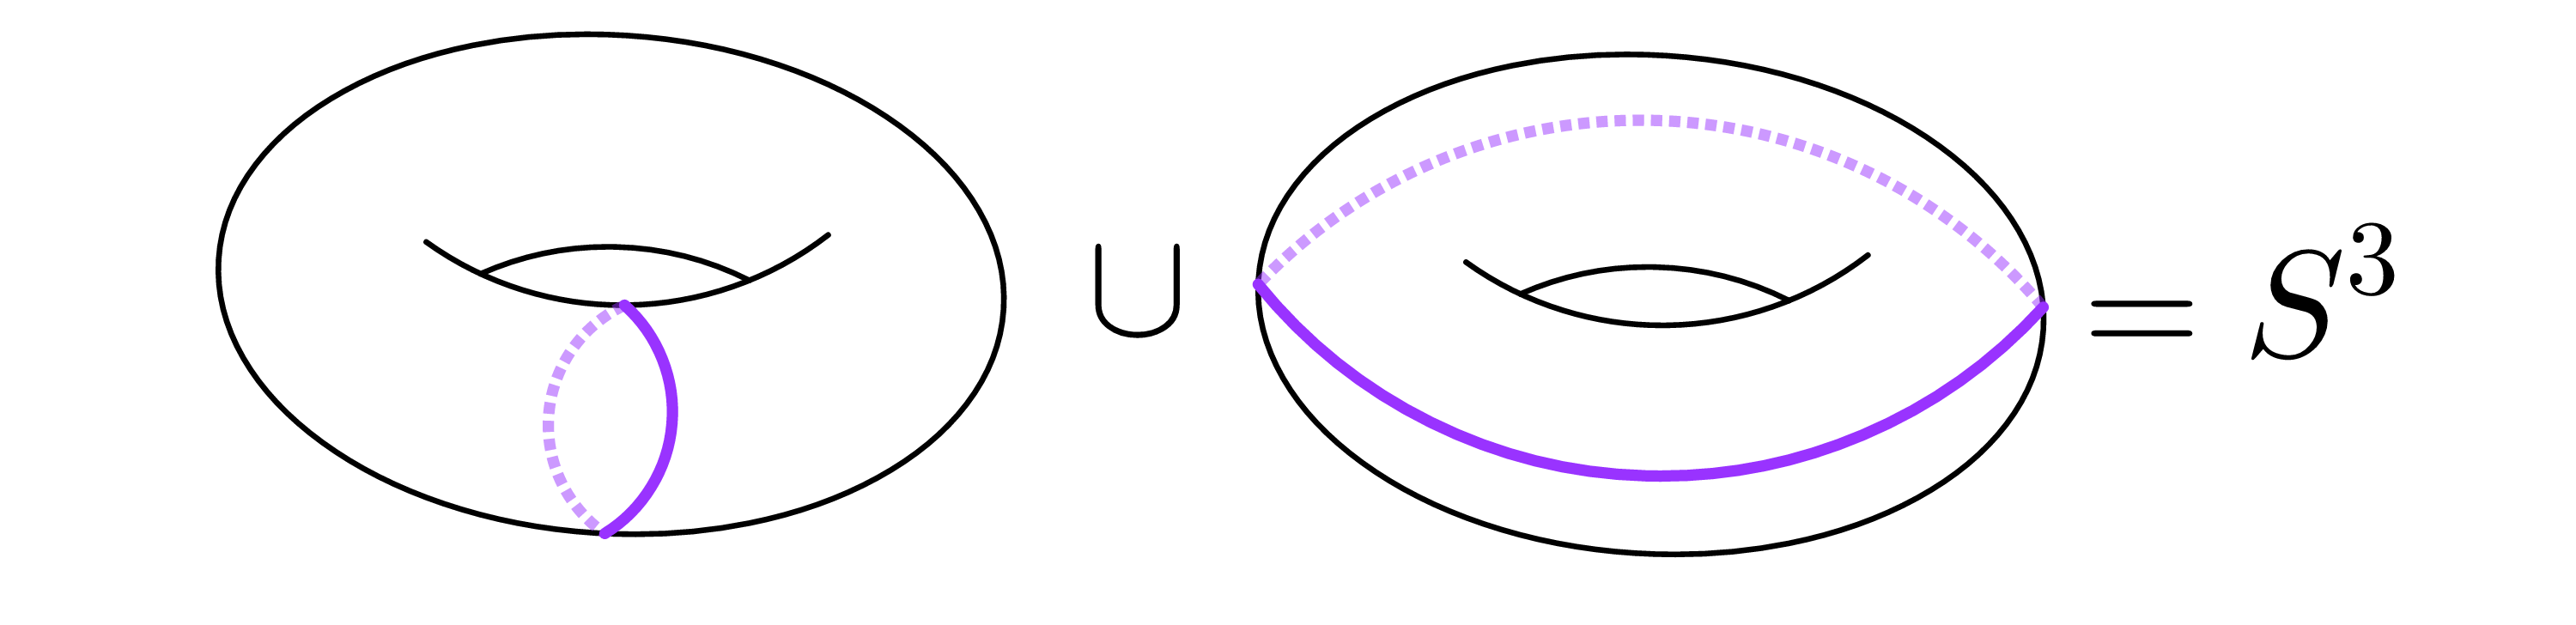
\includegraphics[width=\textwidth]{figures/genus-1-split.png}
	\caption{
		\textbf{Genus 1 Heegaard splitting of $S^3$.}
		The purple curve is essential in each solid torus pictured.
		In the left torus it is a meridian, on the right a longitude.
	}
	\label{fig:genus-1-split}
\end{figure}

\begin{ex}
	The 3--sphere $S^3$ has two standard Heegaard splittings.
	The first is the genus 0 splitting, which is realized by considering $S^3$ as the set of unit vectors in $\R^4$.
	Take the Heegaard surface to be the intersection of $S^3$ with the $xyz$--hyperplane in $\R^4$.
	This is a copy of $S^2$ that separates $S^3$ into two connected components.
	This splitting is written $(S^3,S^2)$
	
	The second is the genus 1 splitting, which is visualized using the realization of $S^3$ as the one--point compactification of $\R^3$.
	Take solid tori $U$ and $V$ and identify $\pd U$ with $\pd V$ by the homeomorphism that swaps a meridian with a longitude.
	The adjunction is $S^3$, and this splitting is written $(S^3,T^2)$.
	Figure \ref{fig:genus-1-split} displays the tori of the splitting.
	This description of $S^3$ is also obtained by examining the boundary of a 4--dimensional 2--handle $\pd (D^2\times D^2)$.
\end{ex}

\begin{defn}
	Let $(M,H)=U\cup_f V$ be a Heegaard splitting of $M$.
	The connected sum $(M,H)\#(S^3,T^2)$ is called an \emph{elementary stabilization} of $M$, and itself is a splitting $(M,H\#T^2)$.
	A Heegaard splitting $(M,H)$ is called a \emph{stabilization} of another splitting $(M,H')$ if it obtained from $(M,H')$ via a finite number of elementary stabilizations.
\end{defn}

Consider the meridians of the solid tori in the standard genus 1 splitting of $S^3$.
They each bound a disc in their respective handlebody, and they intersect in exactly one point.
We would expect to be able to find such curves in any 3--manifold obtained as a stabilization.

\begin{defn}	
	Let $(M,H)=U\cup_f V$ be a Heegaard splitting of genus $g$ and let $\alpha$, $\beta$ a pair of simple, closed, essential curves in $H$.
	Let $\alpha$ be a meridian of $U$ and $\beta$ be a meridian of $V$ with associated meridinal discs $D_\alpha$, $D_\beta$.
	If $\alpha$ and $\beta$ intersect exactly once, then the pair $(\alpha,\beta)$ is a \emph{meridinal pair} or \emph{destabilizing pair} of the splitting.
\end{defn}

To see why $(\alpha,\beta)$ would be called a destabilizing pair, remove a tubular neighbourhood of $D_\alpha$ from $U$ and add it to $V$ as a 2--handle along a tubular neighbourhood of $\alpha$ in $H$.
In fact, the altered spaces $U'$ and $V'$ are handlebodies of genus $g-1$ with $H'= \pd U' = \pd V'$, and $(M,H)$ is a stabilization $(M,H')\#(S^3,T^2)$.
We say that $(M,H')$ is a \emph{destabilization} of $(M,H)$ over $(\alpha,\beta)$.
Note that when we consider $\beta$ to be the belt sphere of a 1--handle and $\alpha$ to be the attaching sphere of a 2--handle, a destabilization is also a handle cancellation.

%This result is summarized in the following lemma (cf.\ Remark 4.2 in \cite{SchlWald}).
%
%\begin{lem}
%	\label{lem:lilwald}
%	Let $M$ be a closed, orientable 3--manifold with a Heegaard splitting $(M,H)$ of genus $g$.
%	If there is a collection of $g$ disjoint destabilizing pairs in $H$, then $M$ is homeomorphic to $S^3$.
%\end{lem}


